%
% Szakdolgozatminta az Eszterházy Károly Katolikus Egyetem
% matematika illetve informatika szakos hallgatóinak.
%

\documentclass[
% opciók nélkül: egyoldalas nyomtatás, elektronikus verzió
% twoside,     % kétoldalas nyomtatás
% tocnopagenum,% oldalszámozás a tartalomjegyzék után kezdődik
]{thesis-ekf}
\usepackage[T1]{fontenc}
\usepackage{hulipsum}
\PassOptionsToPackage{defaults=hu-min}{magyar.ldf}
\usepackage[magyar]{babel}
\usepackage{mathtools,amssymb,amsthm,pdfpages}
\footnotestyle{rule=fourth}

\newtheorem{tetel}{Tétel}[chapter]
\theoremstyle{definition}
\newtheorem{definicio}[tetel]{Definíció}
\theoremstyle{remark}
\newtheorem{megjegyzes}[tetel]{Megjegyzés}

\begin{document}
	\institute{Matematikai és Informatikai Intézet}
	\title{Programozható elektronikák alkalmazásai}
	\author{Bagoly Gábor\\programtervező informatikus}
	\supervisor{Dr. Geda Gábor\\egyetemi docens}
	\city{Eger}
	\date{2023}
	\maketitle
	\tableofcontents
	
	\chapter*{Bevezetés}
	\addcontentsline{toc}{chapter}{Bevezetés}
	
	A mai világunkban az okos otthonok és az okos eszközök rendkívül népszerűek és elterjedtek lettek. Általában, hogy ha megkérdezünk valakit ezzel a témával kapcsolatban, akkor nagy valószínűséggel azt tudják elmondani, hogy rendelkeznek legalább egy okos otthonban alkalmazható eszközzel.
	
	Az okos otthonok és az okos eszközök lehetővé teszik a tulajdonosaik számára, hogy akár távolról is vezéreljék és felügyeljék az otthonukat. Ezek az eszközök lehetővé tehetik a kényelmesebb és hatékonyabb életmód megvalósítását.
	
	Manapság már ha valaki az interneten rákeres valamilyen otthoni eszközre, és eléje írja azt hogy ,,okos'', akkor bizonyára léteznek már erre megoldások. - például okos WC-k, okos kenyérpirítók, még akár okos szőnyegek is, és még sorolhatnám ezt a listát tovább. 
	
	De mi is tesz egy eszközt okossá? Feltételezhetjük azt, hogy ha valami internetre kapcsolódik, esetleg távolról beállíthatjuk, vagy automatizálhatjuk előre meghatározott dolgokra, akkor azt az eszközt ,,okosnak'' tudjuk mondani.
	
	Hogy ha valaki már rendelkezik több ilyen eszközzel, akkor bizonyára találkoztak már azzal a problémával, hogy az egy bizonyos ökoszisztémában használatos eszközök nem feltétlenül tudnak működni egy másikban. Minderre próbáltam egy olyan megoldást kitalálni, ami abból a szempontból közelíti meg, hogy még egy 'nem okos' eszközt (például egy izzót) integrálok bele úgy a rendszerbe, hogy ezt egyszerűen tudjunk kezelni bárhonnan az otthonunkból, ehhez társulva különböző programozható elektronikák. Mindehhez egy olyan webes alkalmazást hoztam létre, amely felelős a háttérben lévő folyamatok lebonyolítására, és az általunk ismert legtöbb eszközön alkalmazható, amin internetezni is tudunk: legyen az számítógép, Androidos, vagy iOS-es telefon, tablet, vagy akár okos óra is.
	
	Azért került erre a témára a választásom, mivel számomra felettébb érdekes az, hogy egy ilyen okos otthonban az eszközök hogyan is kommunikálnak, és szeretnék ebbe egy belátást nyerni, hogy hogyan is épül össze mindez.

	Célom az lenne ezzel, hogy belelássak egy ilyen rendszer működésébe, különböző programozható eszközök alkalmazását jobban megismerjem, és, hogy egy olyan általános kezelőfelületet tudjak létrehozni, amit könnyen tud a felhasználó alkalmazni.
	
	\chapter{Piacon lévő nagyobb okos otthon rendszerek}
	\section{Nagyobb cégek által létrehozott ökoszisztémák}
	Az okos otthon rendszerek széles választéka áll rendelkezésre a piacon felhasználók számára, amelyek között egyszerű rendszerektől kezdve a biztonsági kamerák, ajtózárak és akár a háztartási készülékek is alkalmazhatóak. Amikor az okos otthon rendszer kiválasztására kerül sor, fontos figyelembe venni az eszközök kiválasztását is.
	
	Van néhány olyan eszköz, - például okos izzók vagy okos dugaljak -, amelyek több okos otthon rendszerrel is szabadon használhatóak, így könnyen integrálhatóak a választott rendszerbe. Ezek az eszközök általában ipari szabványokat használnak, mint például a Wi-Fi, Bluetooth LE vagy a Zigbee\footnote{Zigbee-t használ például az Amazon Echo, az IKEA okos otthon termékei, és a Philips Hue}, ami lehetővé teszi számukra, hogy kommunikáljanak a különböző okos otthon rendszerekkel. 
	
	Azonban vannak olyan eszközök is, amelyek kifejezetten egyetlen rendszerrel működnek együtt. Ezek az eszközök saját protokollokat vagy szoftvereket használhatnak, amelyek nem kompatibilisek más rendszerekkel, ami korlátozhatja az okos otthon rendszerünk rugalmasságát. Vegyük példának azt, hogy ha olyan okos ajtózárat vásárlunk, amely csak egy meghatározott okos otthon rendszerrel működik együtt, akkor az eszközt később nem tudjuk használni egy másik rendszerrel. Vagy hogy ha veszünk egy adott típusú eszközt, akkor azt későbbiekben nem tudjuk kombinálni egy másik rendszer eszközével.
	
	Összességében az okos otthon eszközök kiválasztásakor fontos figyelembe venni a kompatibilitást választott okos otthon rendszerünkkel. Az iparági szabványokat támogató eszközök általában rugalmasabbak és szélesebb körű rendszerekkel használhatóak, míg a saját protokollokat használó eszközök korlátozottabbak lehetnek a kompatibilitás terén.
		
	\subsection*{Felvezető: Mik is a virtuális asszisztensek?}
	Virtuális asszisztensek olyan szoftver programok, amik különböző feladatokat tudnak elvégezni számunkra, amit például egy elő segéd is képes lenne. Annyi különbséggel, hogy ezek az asszisztensek online, vagy az eszközeinken léteznek. 
	
	Úgy lettek megalkotva, hogy a felhasználó hang vagy chat alapon tudjanak szimpla kérdésekkel kommunikálni és utasításokat adni. A virtuális asszisztensek olyan feladatokban tudnak segíteni, mint emlékeztetők létrehozása, üzenetek küldése, hívások indítása, internetes keresés, időjárás előrejelzések felolvasása, okos otthoni eszközök irányítása, és egyéb más dolgok. 
	
	Számos cég hozott már létre magának virtuális asszisztenst, amik közül a legismertebbek lehetnek a Google által létrehozott Google Asszisztens, Apple-nek Siri, Amazon-nak Alexa, Samsung Bixby-je, és Microsoft Cortana-ja.
	
	\subsection*{Amazon rendszere - Alexa Smart Home}
	2014-ben lépett be be a piacra az Amazon - \emph{az akkor még újdonságnak számító} - okos hangszórójukkal, az Amazon Echo-val. Ekkor még leginkább csak annyira volt képes, hogy a felhasználó zenét tudja irányítani hang utasításokkal. Ez az eszköz úgy működik, hogy ebbe bele van integrálva az Amazon sajátos virtuális asszisztense, amit Alexának hívnak. Ugye mint kezdetleges szoftver, neki sem voltak a képességei túl szerteágazóak. Leginkább arra tudta az ember használni, hogy egyszerű kérdéseket tegyen fel az ember, és zenét tudjon elindítani, leállítani átugrani.
	
	Nem is annyira később, amikor elkezdett egyre jobban fejlődni Alexa, úgy egyre több mindenre kezdhette el használni az ember: termosztátok beállítása, izzók ki- és bekapcsolására is már lehetett használni. Miután az Amazon egyre többet fektetett bele a rendszerükbe felettébb szerteágazó lett annak a használata az otthonokban. Még arra is volt lehetőség már ekkor, hogy akár bevásárló listát készítsen, és azokat meg is tudja rendelni a felhasználó az Amazonról, mindezt Alexa használatával. A cég 2017 május 23-án jelentette be, hogy a \emph{Smart Home Skill API}-jukba\footnote{A blog poszt amiben bejelentették a Smart Home Skill API bővítését\cite{amazon-api}} innentől kezdve megadható, hogy milyen eszközöket is csatlakoztatunk a rendszerükbe, ami kitárta a lehetőségeket az otthoni okos készülékek automatizációjára. Mindez vezetett az okos otthon piac és a virtuális asszisztensek szerepének növekedéséhez.
	
	Eszközök leginkább hangvezérléssel irányíthatóak, miután követtük az általuk biztosított használati útmutatót. Néhány esetben az Amazon Alexa alkalmazás elegendő lehet, de ha olyan eszközt szeretnénk használni, amelyhez saját alkalmazás tartozik, akkor azt is le kell töltenünk.
	
	Az Amazon által szolgáltatott okos otthon rendszer 2023-ra olyan népszerűségi szintre jutott, hogy az Amerikai Egyesült Államokban az ilyen hang vezérelt hangszórók 68.2\%-a az Amazon Echo.\footnote{Statisztikai adatokat az Earthweb: ,,How Many People Use Alexa in 2023? (U.S. Amazon Statistics)'' cikkjéből \cite{amazon-stats}} Mindezzel napjainkban több ezer eszköz használható már ezen a rendszeren belül: legyen az biztonsági rendszer, háztartási gépek, vagy esetleg szórakoztató rendszerek. Érthető is, hogy sokan miért is szeretik ezt a rendszert használni.
	
	Azonban ennek a rendszernek is megvannak azok a hátulütői, hogy nem minden eszközt tudjunk beintegrálni az adott okos otthon rendszerünkbe, amik nem támogatottak az Amazon által. Érdemes arra odafigyelni, hogy amikor egy okos eszközt veszünk, hogy arra fel-e van tüntetve, hogy kompatibilis az Amazon rendszerével. Másik ilyen negatív tényező lehet számunkra az is, hogy az Amazon Alexa nem használható magyar nyelvvel.
	
	\subsection*{Google rendszere - Google Home és Google Nest}
	
	Az Amazon Echo sikere után a Google is részesülni akart az okos otthon piacának sikereivel. Az akkor még Nest Labs által készült termékek olyanok voltak mint az alkalmazkodó termosztát - amit 2011-ben hoztak létre ,,Nest Learning Thermostat''\footnote{Magyarul: Nest Tanuló Termosztát} néven, ami Wi-Fi-re kapcsolható volt, és szenzorok segítségével alkalmazkodhatott a beltéri hőmérsékleti körülményekre. Ezt követte a következő termékük, a füst és szén-monoxid érzékelő, aminek a neve ,,Nest Protect'' volt. 2014-ben felvásárolták a Dropcam nevezetű céget ami biztonsági kamerákat készítettek, amik után a Nest Labs ezt követő terméke a Nest Cam volt 2015-ben. A Nest Labs egyre jobban látszódó sikerének köszönhetően a Google felvásárolta 2014 januárjában. 2018-ig még önállóan működött a Nest, ami után beolvasztották a Google otthoni termék családba, ezzel létre hozva a Google Nest termékcsaládot, ami számos termékekkel rendelkezik mostanára: termosztát, ajtócsengő, ajtózár, biztonsági kamera, virtuális asszisztenssel integrált érintőképernyős központi egység.\footnote{\label{google-store} További jelenleg elérhető Google Nest családba tartozó termékek: \url{https://store.google.com/gb/category/connected_home} oldalon megtalálható}
	
	Az Amazon Echo-hoz hasonló első terméke a Google-nek a Google Home volt, amit 2016 októberében jelentettek be. Ez a cég sajátos virtuális asszisztensével a Google Assistant-tel volt felszerelve, és ugyan úgy lehetett neki utasításokat adni, és kérdéseket feltenni. Azóta már több otthonon belül alkalmazható eszköz elérhető egyenesen a Google Store-ból.\footref{google-store} Vagy egyéb támogatott harmadik felek által készített ilyen eszközökkel.
	
	Az egyik legnagyobb előnye a Google Home rendszernek az integrációja más Google szolgáltatásokkal, mint például a Google Térkép, a Google Naptár és a Google Fotók. Ez azt jelenti, hogy a felhasználók kéz nélkül is hozzáférhetnek személyes információikhoz és ütemtervükhöz, egyszerűen csak a Google Asszisztensnek kérdést feltéve.
	
	A Google Home rendszer másik erőssége az, hogy képes felismerni a különböző hangokat, amely lehetővé teszi a személyre szabott válaszokat és információkat minden háztartási tag számára. Ez különösen hasznos lehet több személyes háztartásokban, ahol több ember is használja a rendszert.
	
	Összességében a Google Home rendszer egy erős és rugalmas okos otthoni megoldás, amely számos funkciót és lehetőséget kínál. Az integrációja más Google szolgáltatásokkal és a széles körű, kompatibilis eszközökkel rendelkezése miatt a Google Home rendszer erős versenytársa a okos otthoni piacnak.
	
	Viszont a Google Home-nak is meg vannak azok a hátrányai mint az Amazon rendszerének. Sajnos inkább csak akkor tudjuk kihasználni ennek a rendszernek az előnyét, ha angolul vagy más támogatott nyelven beszélünk vele, amibe nem tartozik bele a magyar.
	
	\subsection*{Xiaomi rendszere - Mi Home}
	
	A Xiaomi 2015 júniusában dobta piacra első okos otthon termékcsomagját, a ,,Smart Home Kit''-et, amely mozgásérzékelőt, lámpát és kapacitív kapcsolót tartalmazott. Ezeket az eszközöket egy alkalmazás segítségével lehetett vezérelni, ami lehetővé tette a felhasználók számára, hogy testre szabott utasításokat állítsanak be, például hogy a mozgásérzékelő észlelésekor a lámpa felkapcsoljon, vagy értesítést küldjön a felhasználónak, illetve a csomag támogatta a Xiaomi biztonsági kameráját is. \cite{xiaomi-home}
	
	Ma a Xiaomi okos otthon termékpalettája rendkívül sokrétű, a forrólevegős sütőktől, a robotporszívókon, és a szobamérlegeken át a hőmérséklet- és páratartalom-szenzorokig. Az összes termékük integrálható a Mi Home alkalmazásba, és a felhasználók harmadik féltől származó eszközöket is csatlakoztathatnak hozzájuk. A Xiaomi termékeivel akár komplett otthoni biztonsági rendszert is létre lehet hozni.
	
	Nagy előnye a Xiaomi okos otthon termékeknek az, hogy viszonylag olcsóbb a konkurenciától, és fel is használható például a Google Home, és az Amazon Alexa Smart Home rendszeren belül is, és használata felettébb felhasználó barát.
	
	Kisebb hátránya lehet neki az, hogy ezeket az eszközöket nem lehet asztali alkalmazáson keresztül irányítani, csak is az Androidos és iOS-es alkalmazáson keresztül, vagy esetleg a Google Home vagy Alexa Smart Home-on belül. Amazon Alexával a párosítás mostanában sajnos nehézkesebb, mivel valamilyen oknál fogva nagy százalékban nem tud csatlakozni valami hibánál fogva. Még olyan is megesik, hogy nem minden eszköz érhető el például a Google Home felületen, ilyen lehet példának a biztonsági kamerájuk, ami csak a saját alkalmazásukon érhető el. És mint az előző kettő rendszernél, ez sem használható magyar nyelven.
	
	\section{Nyílt forrású, szabadon személyre szabható rendszerek}
	\subsection*{Mit jelent az, hogy open source?}
	
	Open source, azaz nyílt forráskódú szoftver az olyan, aminek a forráskódját szabadon lehet vizsgálni, módosítani, és akár ki is egészíteni. A kód az a része egy szoftvernek amit a legtöbb felhasználó bizonyára soha nem fog látni. Ez az a kód, amit a programozók változtathatnak hogy megváltozzon a program vagy alkalmazás működése. Azok a programozók, akik hozzáférhetnek egy szoftver forráskódjához, azokat feljeszthetik, és javíthatják azzal hogy például új funkciót adnak hozzá, vagy kijavítanak egy olyan részt, ami nem minden esetben működik helyesen.\footnote{\label{open-source-fn}A nyílt forráskódú szoftverről az irodalomjegyzék \cite{what-is-open-source}. részén található}
	
	Azonban azt, hogy egy szoftver nyílt forráskódú, nem feltétlenül jelenti azt, hogy az adott szoftver ingyenes használatban áll. Nyílt forráskódot fejlesztő programozók kérhetnek pénzt azért a nyílt forrású szoftverért, hogy ha ők alkották meg, vagy hozzájárulásukkal készült el. 
	
	Bizonyos esetekben azonban, mivel a nyílt forráskódú licenc megkövetelheti a program forráskódjának kiadását amikor szoftvert adnak el másoknak, egyes programozók úgy találják, hogy jövedelmezőbb pénzt kérni a felhasználóktól a szoftverszolgáltatásokért és - támogatásért (nem feltétlenül magáért a szoftverért). Így a szoftvereik ingyenesek maradnak, és pénzt keresnek azzal, hogy másoknak segítenek telepíteni, használni és hibaelhárítást végezni.\footref{open-source-fn}
	
	\subsection*{Home Assistant}
	
	A Home Assistant 2013 novemberére került publikálásra \emph{GitHub.com}-on \textsc{Paulus Schoutsen} által. Ez ekkor még egy Python programozási nyelven megírt alkalmazás volt. Ekkor még ez egy egyszerű program volt, ami napnyugtakor felkapcsolta a lámpát. Azóta a szoftver elég érett lett, és körülbelül 20 aktív hozzájáruló dolgozik a projekten, ennek köszönhetően kéthetente érkezik frissítés a rendszerre.\footnote{\label{history-of-home-assistant}A történet bővebben az irodalomjegyzék  \cite{creation-of-home-assistant}. részén megtalálható.}
	
	Ez a szoftver bármely olyan rendszeren működik, ami a Python 3 programozási nyelvet tudja futtatni. Biztosít mobil és számítógép alkalmazást is, mellyel több ezer támogatott eszközt tudunk irányítani. Annyi a különbség ez a rendszer és a nagyobb cégek által biztosított között, hogy ez teljesen lokálisan fut, és hogy ha esetleg internet kimaradás lenne, még akkor is tudjuk ugyan úgy irányítani eszközeinket. A rendszer által számos ismert okos eszköz támogatott, mint például a Philips Hue, IKEA TRÅDFRI, és akár az Amazon Echo, Google Home, és a Xiaomi Mi Home által támogatott eszközök, és még a virtuális asszisztensük is.\footnote{A támogatott rendszerek a weboldalukon elérhető, ami az irodalomjegyzék \cite{home-assistance-itegrations}. részén megtalálható} Mindez annak köszönhető, mert Z-Wave és a Zigbee protokoll is támogatott a rendszer által, és mivel nyílt forráskódú a szoftver, ezért bármikor lehet az hogy valamelyik felhasználó vagy esetleg fejlesztő hozzáadja bizonyos termékeket kiegészítésként. 

	A rendszerrel háztartásunk energiafelhasználását is nyilván lehet tartani. Szabadon testre szabható a felület kinézete a felhasználók ízlése szerint. Szintén pozitívum lehet, hogy az szoftver támogatja a magyar nyelvet is.
	
	Ámbár ez a rendszer azoknak ajánlott jobban, akik informatika terén ismertek.
	
	\subsection*{OpenHAB}
	
	OpenHAB, azaz Open Home Automation Bus\footnote{Magyarul: Nyílt Otthon Automatizációs Busz} fejlesztése 2010-ben kezdődött, és Java programozási nyelvben lett megírva. 2013-ban került elérhetővé az első stabil verziója a szoftvernek. 
	
	Az OpenHAB legelső körben azon a személyek számára ajánlott, akik jól ismertek informatika, és robotika terén. Ez azért szükséges, mert nekünk kell összeállítanunk, hogy mit szeretnénk elérni az okos otthon rendszerünkben. Az alkalmazás rendkívül rugalmas és testre szabható, és nagy a támogatottsága. Ez az egyik legelterjedtebb nyílt forráskódú okos otthon rendszer, és folyamatos fejlesztés alatt áll egy nonprofit szervezet által, aminek a fejlesztésébe bárki beállhat.
	
	Ez a rendszer képes integrálni a piac különböző eszközeit, mint ahogyan azt a Home Assitant rendszernél is említettem. Szintén egy fontos tényezője, hogy lokálisan működik, ezért egy internet kimaradásnál az okos otthonunk ugyan úgy működni fog. 
	
	A szoftvernek hivatalos oldalon megtalálható a teljes dokumentációja, hogy mit hogyan kell összeállítani és használni, ezért lehet kedvelt olyan személyek számára, akik szeretik a dolgokat maguknak összeállítani. A rendszer nagy támogatást és közösséget élvez, így ha felmerülne bármilyen kérdés, biztosan választ kapunk rá.
	
	Az ezzel létrehozott otthonunkat a legtöbb felületen el tudjuk érni, legyen az MacOS, Windows, Linux, Android vagy iOS.
	\footnote{Az OpenHAB hivatalos oldala megtalálható a az irodalomjegyzék \cite{openhab}. részén, ahol olvasható a dokumentációjuk, a céljaik, és egyéb blogjaik.}
	
	%----------
	\chapter{Alkalmazott eszközök}
	\section{Hardver}
	\subsection{Raspberry Pi 4B}
	\subsection{ESP-Wroom-32 - Wi-Fi-s Mikrokontroller}
	\subsection{ESP32-CAM - Wi-Fi-s kamera modul}
	\subsection{DHT22 - hőmérséklet és páratartalom szenzor}
	\subsection{RFID-RC522 - RFID olvasó + RFID technológia összefoglaló}
	\subsection{Szolidtest relé}
	\subsection{Eszközök bekötése - Fritzing}
	
	\section{Szoftver - Programozási nyelvek}
	\subsection{C++ - Arduino IDE}
	\subsection{HTML - PHP Storm}
	\subsection{PHP - PHP Storm}
	\subsection{JavaScript, ChartJS, jQuery - PHP Storm}
	\subsection{Tailwind}
	\subsection{dbDiagram}
	\subsection{font-awesome}
	\subsection{MySQL}
	\subsection{plantUML}
	\section{Laravel}
	\subsection{Laravel működése}
	%----------
	
	\chapter{A web alkalmazás felépítése és működése}
	\section{Raspberry PI4B alkalmazása, mint Wi-Fi, és hub}
	\section{Adatbázis felépítése}
	\section{Kezelő felület bemutatása és működése}
	\subsection{Főoldal}
	\subsection{Beállítások}
	\subsection{RFID beállítások}
	\subsection{RFID használati táblázat}
	\subsection{Hőmérsékleti és páratartalom előzmények - ChartJS}
	\section{Eszközök kommunikációja a webszerverrel}
	
	%----------
	\chapter{Tesztelések}
	\section{Tesztelések módjai és fontossága}
	
	\subsection{Cypress automatizált tesztelések}
	\subsection{Manuális tesztelések}
	\begin{table}[h]
		\centering
		\begin{tabular}{|p{6cm}|p{6cm}|p{4cm}|}
			\hline
			\textbf{Teszt leírása} & \textbf{Elvárt eredmények} & \textbf{Tapasztalatok} \\
			\hline
			Access Control Test: RFID tags assigned to users &
			 The system should recognize the RFID tags assigned to each user and grant or deny access to specific devices or areas of the home accordingly &
			  The test was successful, with the system accurately recognizing and responding to each user's assigned RFID tag \\
			\hline
			Device Control Test: Using RFID tags to control devices &
			 The system should allow users to control smart home devices (such as lights or locks) using RFID tags, without requiring additional input &
			  The test was partially successful, with the system accurately recognizing the RFID tags but experiencing some delays in device response times \\
			\hline
			Durability Test: RFID tags in high traffic areas &
			 The RFID tags should remain functional and readable even in high traffic areas, with no degradation in performance &
			  The test was successful, with the RFID tags remaining fully functional and readable even with heavy usage \\
			\hline
			Security Test: Unauthorized access prevention &
			 The system should be designed to prevent unauthorized access by detecting and alerting the user to the presence of unrecognized RFID tags & 
			 The test was successful, with the system detecting and preventing access by an unrecognized RFID tag, and sending an alert to the user's mobile device \\
			\hline
		\end{tabular}
		\caption{Manuális tesztelések a webalkalmazásra}
		\label{table:manual-testing-results}
	\end{table}
	
	%----------
	\chapter{Rendszer telepítése}

	
	\chapter*{Összegzés}
	\addcontentsline{toc}{chapter}{Összegzés}
	
	\begin{thebibliography}{20}
		\addcontentsline{toc}{chapter}{\bibname}
		
		\bibitem{amazon-api}
		\textsc{Jeff Blankenburg}: \emph{Define Your Appliance Category for a Better Customer Experience}\\
		\textsc{URL:} \url{https://developer.amazon.com/blogs/alexa/post/a89f7243-08a0-4c73-8fc5-eb604a93f437/define-your-appliance-category-for-a-better-customer-experience}\\
		\textsc{Link utoljára ellenőrizve:} 2023.03.31.
		
		\bibitem{amazon-stats}
		\textsc{Jason Wise}: \emph{How Many People Use Alexa in 2023? (U.S. Amazon Statistics)} \\
		\textsc{URL:} \url{https://earthweb.com/alexa-users/}\\
		\textsc{Link utoljára ellenőrizve:} 2023.03.31.
		
		\bibitem{xiaomi-home}
		\textsc{HandWiki}: \emph{Engineering:Xiaomi Smart Home}
		\textsc{URL:} \url{https://handwiki.org/wiki/Engineering:Xiaomi_Smart_Home}\\
		\textsc{Link utoljára ellenőrizve:} 2023.03.31.
		
		\bibitem{what-is-open-source}
		\textsc{What is open source}\\
		\textsc{URL:} \url{https://opensource.com/resources/what-open-source}\\
		\textsc{Link utoljára ellenőrizve:} 2023.03.31.
		
		\bibitem{creation-of-home-assistant}
		\textsc{Eric Brown}: \emph{Home Assistant: The Python Approach to Home Automation}\\
		\textsc{URL:} \url{https://www.linux.com/topic/embedded-iot/home-assistant-python-approach-home-automation/}\\
		\textsc{Link utoljára ellenőrizve:} 2023.03.31.
		
		\bibitem{home-assistance-itegrations}
		\textsc{Home Assistant - Integrations}\\
		\textsc{URL:} \url{https://www.home-assistant.io/integrations/}\\
		\textsc{Link utoljára ellenőrizve:} 2023.03.31.
		
		\bibitem{openhab}
		\textsc{OpenHAB hivatalos oldala}\\
		\textsc{URL:} \url{https://www.openhab.org/}\\
		\textsc{Link utoljára ellenőrizve:} 2023.03.31.
		
		\bibitem{what-is-smarthome}
		\textsc{What is the Smart Home?}\\
		\textsc{URL:} \url{https://shaba.eu/2020/11/03/what-is-the-smart-home/}\\
		\textsc{Link utoljára ellenőrizve:} 2023.03.31.
		
		\bibitem{smart-home-definition}
		\textsc{Forrest Stroud}: \emph{Smart Home}\\
		\textsc{URL:} \url{https://www.webopedia.com/definitions/smart-home/}\\
		\textsc{Link utoljára ellenőrizve:} 2023.03.31.
		
		\bibitem{raspberrypi-4b}
		\textsc{Offical Raspberry Pi 4B dokumentation}\\
		\textsc{URL:} \url{https://www.raspberrypi.com/documentation/computers/raspberry-pi.html#raspberry-pi-4}\\
		\textsc{Link utoljára ellenőrizve:} 2023.03.31.
		
		\bibitem{ESP32-devices}
		\textsc{Offical ESP32 devices documentation}\\
		\textsc{URL:} \url{http://esp32.net/#Info}\\
		\textsc{Link utoljára ellenőrizve:} 2023.03.31.
		
		\bibitem{esp32-wroom}
		\textsc{NodeMCU ESP-WROOM-32 internal details and pinouts}\\
		\textsc{URL:} \url{https://www.instructables.com/ESP32-Internal-Details-and-Pinout/}\\
		\textsc{Link utoljára ellenőrizve:} 2023.03.31.
		
		\bibitem{RFID-card-reader}
		\textsc{Connect RFID to PHP \& MySQL Database with NodeMcu ESP8266}\\
		\textsc{URL:} \url{https://iotprojectsideas.com/connect-rfid-to-php-mysql-database-with-nodemcu-esp8266/}\\
		\textsc{Link utoljára ellenőrizve:} 2023.03.31.
		
		\bibitem{node32-httpget}
		\textsc{ESP8266 NodeMCU HTTP GET and HTTP POST with Arduino IDE (JSON, URL Encoded, Text)}\\
		\textsc{URL:} \url{https://randomnerdtutorials.com/esp8266-nodemcu-http-get-post-arduino/#http-get-1}\\
		\textsc{Link utoljára ellenőrizve:} 2023.03.31.
		
		\bibitem{arduino-to-laravel}
		\textsc{Arduino to Laravel Communication}\\
		\textsc{URL:} \url{https://www.instructables.com/Arduino-to-Laravel-Communication/}\\
		\textsc{Link utoljára ellenőrizve:} 2023.03.31.
		
		\bibitem{raspberry-as-wifi}
		\textsc{Raspberry configuration for Wi-Fi}\\
		\textsc{URL:} \url{https://www.raspberrypi.com/documentation//computers/configuration.html#setting-up-a-routed-wireless-access-point}\\
		\textsc{Link utoljára ellenőrizve:} 2023.03.31.
		
		\bibitem{laravel-docs}
		\textsc{Offical Laravel Documentation}\\
		\textsc{URL:} \url{https://laravel.com/docs/10.x}\\
		\textsc{Link utoljára ellenőrizve:} 2023.03.31.
		
		\bibitem{tailwind-docs}
		\textsc{Offical Tailwind Documentation}\\
		\textsc{URL:} \url{https://tailwindcss.com/docs}\\
		\textsc{Link utoljára ellenőrizve:} 2023.03.31.
		
		\bibitem{chartjs-docs}
		\textsc{Offical Chart.js Documentation}\\
		\textsc{URL:} \url{https://www.chartjs.org/docs/latest/}\\
		\textsc{Link utoljára ellenőrizve:} 2023.03.31.
			
		\bibitem{cypress-docs}
		\textsc{Offical Cypress Documentation}\\
		\textsc{URL:} \url{https://docs.cypress.io/guides/overview/why-cypress}\\
		\textsc{Link utoljára ellenőrizve:} 2023.03.31.
		
		\bibitem{fontawesome}
		\textsc{Fontawesome - Free Icons}\\
		\textsc{URL:} \url{https://fontawesome.com/search?o=r&m=free}\\
		\textsc{Link utoljára ellenőrizve:} 2023.03.31.
				
	\end{thebibliography}
	
	% Aláírt, szkennelt nyilatkozat beillesztése a szakdolgozat végére
	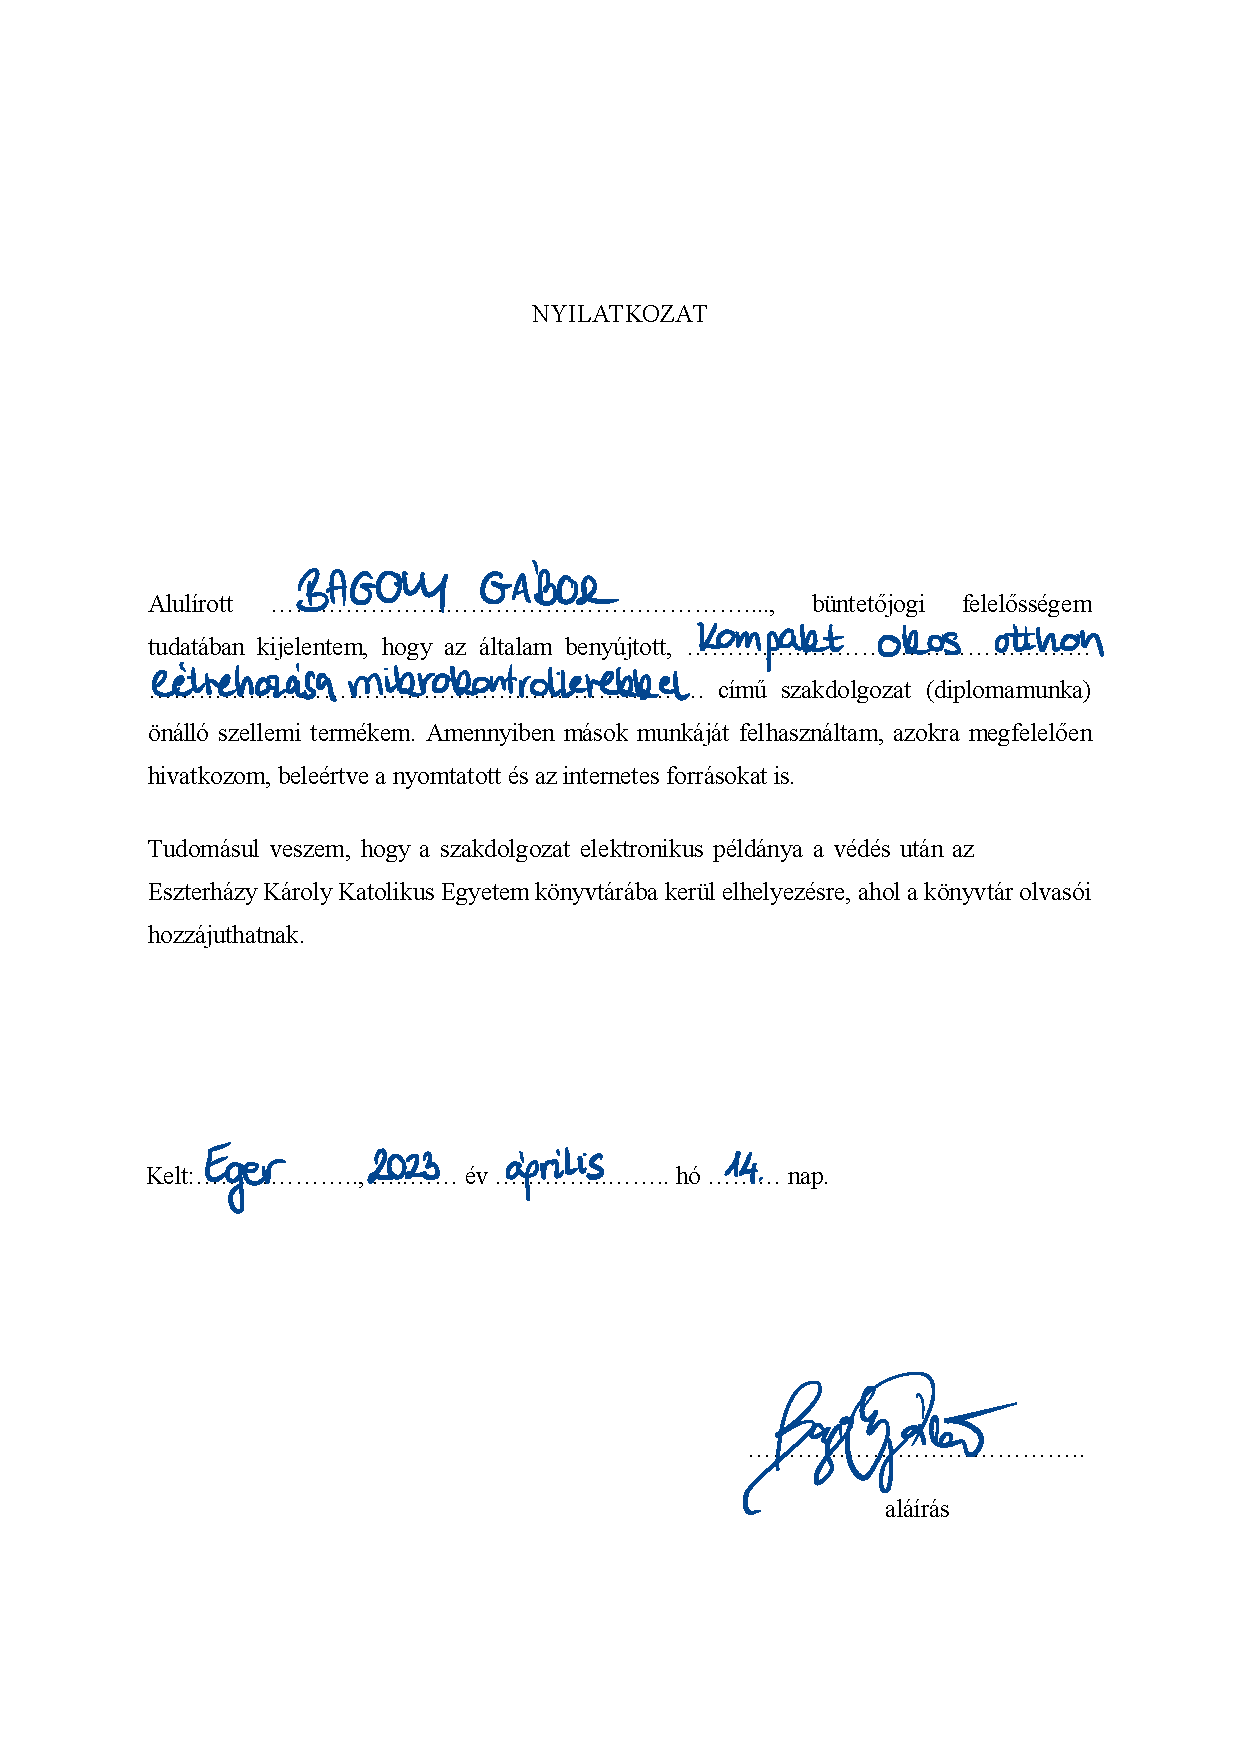
\includepdf{nyilatkozat.pdf}
\end{document}